\section{Results and discussion} \label{s:results}

\subsection{Validation}

\subsubsection{Reflectance and transmittance} \label{sss:refltrans}

\begin{figure}[h] \centering
  \centerline{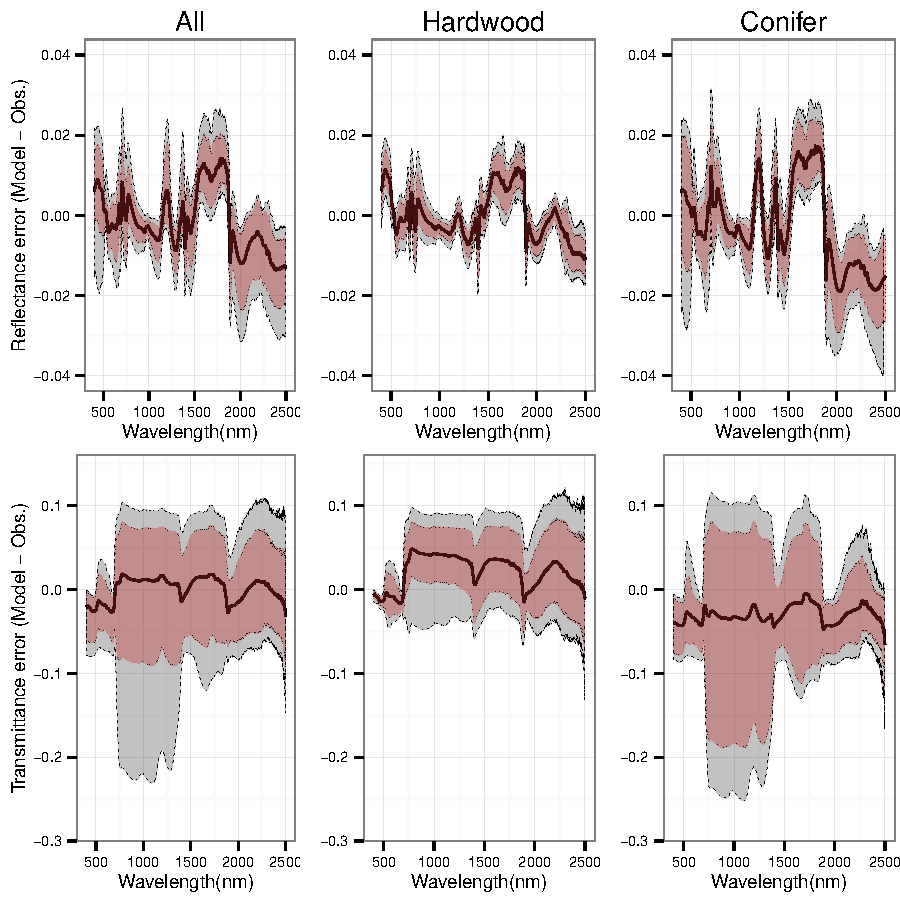
\includegraphics{figures/refltrans-validation}}
  \caption{
    Errors in reflectance (top) and transmittance (bottom) spectra simulated
    using PROSPECT 4 parameters from the inversion output for all leaves(left)
    and only hardwood (middle) and conifer (right) species. For a given
    wavelength, the solid black line is the mean error, the red region bounded
    by the dotted line is the 90\% confidence interval on the error, and the
    grey region bounded by the dashed line is the 95\% confidence interval.
  }
  \label{fig:refltrans}
\end{figure}

Figure \ref{fig:refltrans} shows the results of the validation based on
comparison of observed and simulated reflectance and transmittance spectra.
At the scale of the entire data set, statistically significant reflectance
errors occurred in the near and short wave infrared region, with overestimates
in the \SIrange{1500}{1900}{\nano\meter} range and underestimates at around
\SIlist{1100;2000;2400}{\nano\meter}.  For broadleaved species, significant
differences in reflectance were overestimates around \SI{450}{\nano\meter} and
in the \SIrange{1500}{1900}, while needle-leaved reflectance was overestimated
around \SI{1700}{\nano\meter}.  Other prominent reflectance errors lined up
with spectral ``edges''--i.e.  large changes in reflectance over a small
number of wavelengths, such as the chlorophyll absorption ``green edge'' or
the leaf structural scattering ``red edge''--but none of these errors were
significantly different from zero.

Errors in transmittance were, on average, greater than those for reflectance,
with mean transmittance mostly overestimated for broadleaved species and
underestimated for needle-leaved species. However, the variability in these
errors was also very large, meaning that statistically significant
($p < 0.05$) errors occurred in only a few very specific regions of the spectrum:
Around \SI{450}{\nano\meter}, corresponding to chlorophyll a absorption;
around \SI{700}{\nano\meter}, corresponding to the vegetation ``red edge'';
and, for needle-leaved species, around \SI{1900}{\nano\meter}, corresponding
to a water absorption feature.

Our study is not the first to report issues with modeling reflectance and
transmittance in the \SIrange{400}{450}{\nano\meter} range.  Feret et al.
\cite{Feret2008} observed a consistently negative transmittance bias and
occasionally a positive or negative reflectance bias.  Similarly, Croft et al.
\cite{Croft2013} report systematic underestimates of reflectance in this
region. Most likely, these biases are the result of the failure of the
PROSPECT model to distinguish between chlorophyll a and b, which
have overlapping but distinctly different absorption signatures and whose
ratios have been shown to be affected by environmental conditions
(\cite{Blackburn2007, DiVittorio2009b, DiVittorio2009a}).  Fortunately, it has
been shown that not only can chlorophyll a and b be distinguished using
imaging spectroscopy (\cite{DiVittorio2009a}), but that these differences can
be incorporated into a radiative transfer model to improve its performance
(\cite{DiVittorio2009}).  As such, we argue that future development of
PROSPECT and other radiative transfer models should include this distinction.

The large variability in transmittance errors is most likely driven by the
fact that our inversion procedure targeted only reflectance. If we had used
both reflectance and transmittance data, we would expect to see the
variability distributed more evenly. That being said, the inherent challenges
of measuring transmittance--especially related to the expense and insufficient
quality of integrating spheres--likely contribute to substantially higher
uncertainties in the measured transmittance. This is supported by the absence
of significant systematic bias between measured and modeled transmittance
(except in the regions discussed above).  Furthermore, although the confidence
intervals in Figure \ref{fig:refltrans} appear very large, when averaged over
the visible (\SIrange{400}{800}{\nano\meter}) and infrared
{\SIrange{801}{2500}{\nano\meter}) regions, the resulting statistics are at
least comparable to--and often better than--those reported in other field
spectra inversion studies (Table \ref{tab:refltrans}).  Although our overall
transmittance RMSE values were higher than that reported by \cite{Feret2008},
these errors are inflated by the inclusion of needle-leaved species, whose
reflectance is harder to measure reliably and which do not satisfy the
assumptions of the PROSPECT model.  When looking only at hardwoods, our
statistics for transmittance were fully comparable to \cite{Feret2008},
despite the fact that we did not use any transmittance information to perform
the inversion.  When compared with transmittance error statistics reported for
conifers by \cite{DiVittorio2009}, our values are of very similar magnitude,
even despite the fact that \cite{DiVittorio2009} used the more
needleleaf-friendly LIBERTY model.  Moreover, our reflectance error statistics
are consistently comparable to or lower than those reported in comparable
studies (\cite{Feret2008, DiVittorio2009}.

% latex table generated in R 3.2.1 by xtable 1.7-4 package
% Fri Aug 14 16:30:07 2015
\begin{table}[ht]
\centerline{
\begin{tabular}{rrrrrrr}
  \hline
 & VIS-RMSE & VIS-BIAS & VIS-SEPC & IR-RMSE & IR-BIAS & IR-SEPC \\ 
  \hline
All-R & 0.0077 & 0.0019 & 0.0064 & 0.0095 & -0.0021 & 0.0056 \\ 
  Hardwood-R & 0.0062 & 0.0023 & 0.0040 & 0.0062 & -0.0009 & 0.0030 \\ 
  Conifer-R & 0.0092 & 0.0014 & 0.0079 & 0.0123 & -0.0036 & 0.0057 \\ 
  All-T & 0.0403 & -0.0133 & 0.0335 & 0.0551 & 0.0041 & 0.0536 \\ 
  Hardwood-T & 0.0248 & 0.0012 & 0.0167 & 0.0450 & 0.0266 & 0.0336 \\ 
  Conifer-T & 0.0553 & -0.0345 & 0.0389 & 0.0660 & -0.0291 & 0.0565 \\ 
   \hline
\end{tabular}
}
\caption{ Modeled reflectance (R) and transmittance (T) error statistics. } 
\label{tab:refltrans}
\end{table} 

\subsubsection{EWT and LMA}

Figures \ref{fig:water} and \ref{fig:lma} compare inversion parameter
estimates and direct measurements for equivalent water thickness (EWT;
PROSPECT parameter Cw) and leaf mass per unit area (LMA; PROSPECT parameter
Cm), respectively. Table \ref{tab:water-lma} shows the relevant summary
statistics for both. 

Echoing the results of the spectral validation (section \ref{sss:refltrans}),
parameter estimates were much more accurate for broadleaved than needleleaved
species, and the relevant statistics for broadleaved species agree with those
reported by others (\cite{Feret2008, Li2011a}.  Interestingly, the strongest
overestimates for both EWT and LMA occur in early successional needleleaf
species, which for this data set consisted entirely of pine species
(\textit{Pinus} family). One explanation for this is the unique methodological
challenge of measuring pine needle reflectance using a leaf-clip setup, as
multiple needles are required to completely cover the spectroradiometer lens
and the rounded shape of pine needles (compared to the flatter shape other
conifer families) may artificially dampen the measured reflectance, thereby
leading to parameter overestimation. Alternatively, the overestimation may be
the result of saturation in the response of PROSPECT to its parameters; i.e.
as parameters get larger, it becomes harder to distinguish between them (See
Figure \ref{fig:prospectsens}).  

The persistent negative bias we found in spectral estimates of LMA for
broadleaved species has been reported elsewhere but inconsistently so, with
some studies showing negative bias across all their data (\cite{Li2011a,
Cheng2014}) and others reporting a bias whose magnitude and direction is
data-dependent (\cite{Feret2008}). This may partially be explainable by the
simplicity of PROSPECT's treatment of leaf structural components;
specifically, protein, cellulose, hemicellulose, sugar, starch, and lignin are
aggregated into a single parameter (Cm) (\cite{Fourty1996}) based on the sum
of their absorption features.  As with chlorophyll, this fails to take into
account variability in the relative abundance of the different components,
which varies substantially in response to environmental conditions
(\cite{Poorter2009}).  Furthermore, measurements of LMA are likely to
inadvertently include additional components such as chlorophyll, carotenoids,
lipids, organic acids, phenolics, and vascular tissue (\cite{Poorter2009}),
which would positively bias the measurement compared to the spectral estimate.
Similarly, as a spectral parameter, Cm is driven by the area over which
absorption can take place, which is affected by the geometry of absorbing
structural materials in the leaf and may therefore be slightly larger than the
actual measured leaf area; this would also negatively bias the inversion
estimate.  Finally, it is possible that the inversion is confused by the
significant overlap in the spectral effects of scattering by multiple layers
(N parameter) and absorption by leaf structural components (Cm parameter)
(Figure \ref{fig:prospectsens}), which results in strong positive covariance
in the sampling of these two parameters (Figure \ref{fig:pairs4}).  We are
aware of only one other study that attempted to estimate all five PROSPECT
parameters simultaneously: Li and Wang (\cite{Li2011a}) presented a novel
algorithm for PROSPECT inversion that assigns a separate merit function to
each parameter and demonstrated its improved performance over traditional
approaches.  However, although their new algorithm reduced error and bias in
the LMA estimates, a negative bias comparable to the one we report still
remained across all of their data sets. 

\begin{figure}[h]
  \centering
  \centerline{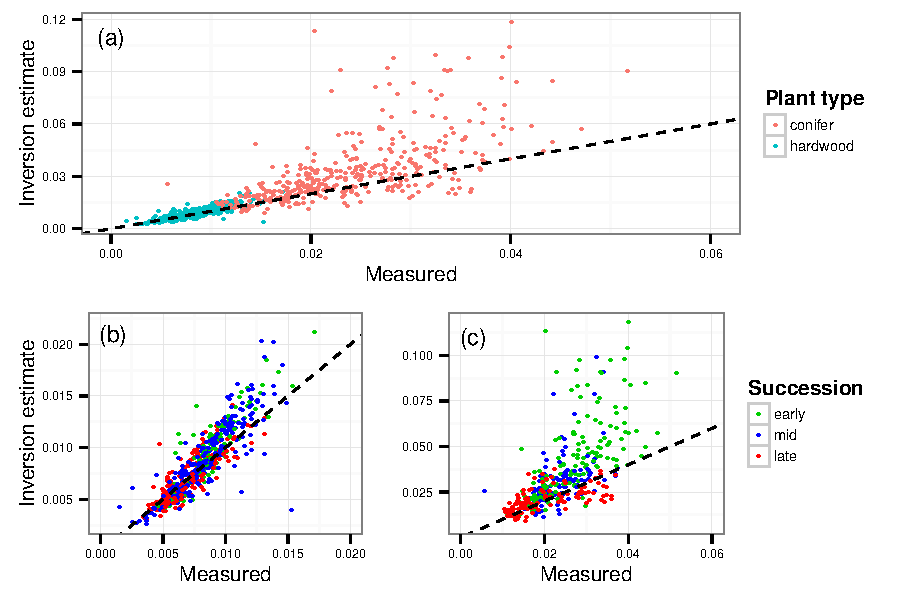
\includegraphics{figures/water}}
  \caption{
    Modeled and observed equivalent water thickness for both conifers and 
    hardwoods (a), just hardwoods (b), and just conifers (c). Point colors 
    indicate plant type (a) or successional stage (b,c). The dashed line 
    represents a 1:1 fit.
    }
  \label{fig:water}
\end{figure}

\begin{figure}[h]
  \centering
  \centerline{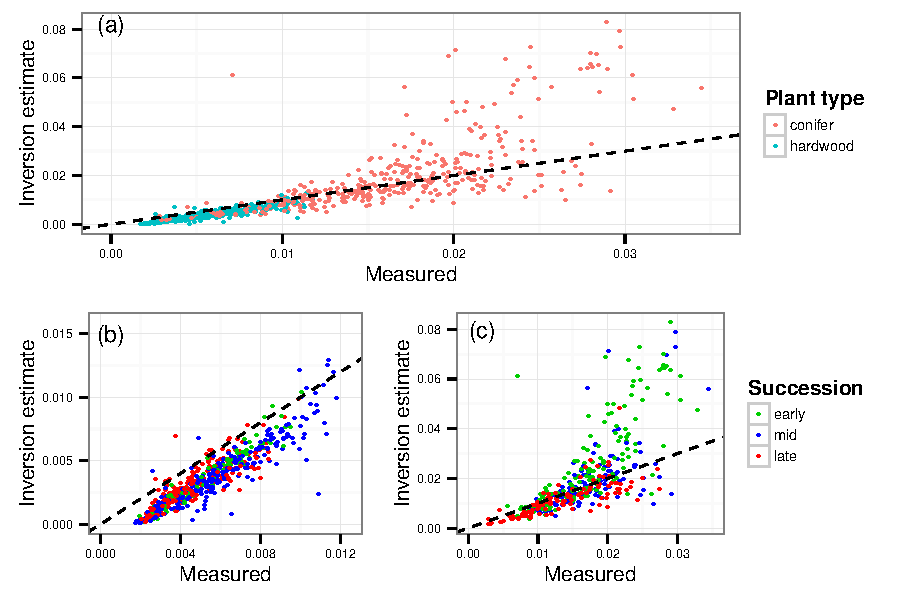
\includegraphics{figures/lma}}
  \caption{
    Modeled and observed leaf mass per unit area (g cm-2) for both conifers 
    and hardwoods (a), just hardwoods (b), and just conifers (c). Point colors 
    indicate plant type (a) or successional stage (b,c). The dashed line 
    represents a 1:1 fit.
    }
  \label{fig:lma}
\end{figure}

% latex table generated in R 3.2.1 by xtable 1.7-4 package
% Fri Aug 14 16:30:08 2015
\begin{table}[ht]
\centerline{
\begin{tabular}{llrrrrr}
  \hline
Parameter & Plant type & RMSE & BIAS & SEPC & CV & RMSPE \\ 
  \hline
EWT & conifer & 0.0191 & 0.0091 & 0.0168 & 0.5324 & 0.6930 \\ 
  EWT & hardwood & 0.0017 & 0.0005 & 0.0016 & 0.1880 & 0.2162 \\ 
  LMA & conifer & 0.0125 & 0.0036 & 0.0119 & 0.6330 & 0.6712 \\ 
  LMA & hardwood & 0.0020 & -0.0018 & 0.0009 & 0.2450 & 0.4375 \\ 
   \hline
\end{tabular}
}
\caption{ Error statistics for equivalent water thickness (EWT) and leaf mass per unit area (LMA) model estimates compared to inversion. } 
\label{tab:water-lma}
\end{table}

\subsection{Effect of sensor}

Table \ref{tab:sensor} summarizes the results of the sensor simulation
experiment by showing the mean inaccuracy and uncertainty for each sensor.

% latex table generated in R 3.2.1 by xtable 1.7-4 package
% Fri Aug 14 16:30:08 2015
\begin{table}[ht]
\centerline{
\begin{tabular}{lrrrrrrrrrr}
  \hline
Sensor & $\pi(\mathrm{N})$ & $\pi(\mathrm{Cab})$ & $\pi(\mathrm{Car})$ & $\pi(\mathrm{Cw})$ & $\pi(\mathrm{Cm})$ & $\alpha(\mathrm{N})$ & $\alpha(\mathrm{Cab})$ & $\alpha(\mathrm{Car})$ & $\alpha(\mathrm{Cw})$ & $\alpha(\mathrm{Cm})$ \\ 
  \hline
ASD Field Spec & 0.0008 & 0.0015 & 0.0065 & 0.0009 & 0.0038 & -0.0001 & -0.0001 & -0.0002 & -0.0001 & -0.0000 \\ 
  AVIRIS NG & 0.0036 & 0.0073 & 0.0339 & 0.0041 & 0.0191 & -0.0021 & -0.0019 & -0.0031 & -0.0019 & -0.0001 \\ 
  AVIRIS Classic & 0.0064 & 0.0138 & 0.0681 & 0.0074 & 0.0358 & -0.0049 & -0.0044 & -0.0088 & -0.0045 & 0.0015 \\ 
  Hyperion & 0.0062 & 0.0138 & 0.0702 & 0.0071 & 0.0356 & -0.0053 & -0.0047 & -0.0030 & -0.0050 & 0.0008 \\ 
  CHRIS-Proba & 0.0000 & 0.0000 & 0.0000 & 0.0000 & 0.0002 & 0.0000 & 0.0000 & 0.0000 & 0.0000 & 0.0000 \\ 
  Landsat 5 & 0.0287 & 0.0560 & 0.2795 & 0.0488 & 0.2011 & -0.0336 & -0.0353 & -0.0278 & -0.0116 & 0.3628 \\ 
  Landsat 7 & 0.0288 & 0.0649 & 0.3196 & 0.0470 & 0.2005 & -0.0344 & -0.0250 & -0.0833 & -0.0152 & 0.3312 \\ 
  Landsat 8 & 0.0242 & 0.0513 & 0.3110 & 0.0477 & 0.1204 & -0.0242 & -0.0222 & -0.0510 & -0.0125 & 0.1736 \\ 
  MODIS & 0.0310 & 0.0466 & 0.5450 & 0.0505 & 0.2453 & -0.0392 & -0.0437 & 0.0896 & -0.0445 & 0.3070 \\ 
  VIIRS & 0.0135 & 0.0408 & 0.4150 & 0.0187 & 0.0726 & -0.0153 & -0.0082 & -0.0938 & -0.0105 & 0.0793 \\ 
  AVHRR & 0.0702 & 0.3045 & 0.7243 & 0.2141 & 0.4815 & -0.0191 & -0.0884 & -0.3566 & -0.0429 & 1.8278 \\ 
   \hline
\end{tabular}
}
\caption{ Mean inaccuracy ($\alpha$) and uncertainty ($\pi$) by sensor. } 
\label{tab:sensor}
\end{table}

\subsubsection{Parameter error}

Figure \ref{fig:sensor-error} compares known parameter values and inversion
estimates for simulated spectra filtered through the spectral response
functions of various sensors. The spectral resolution of the four
hyperspectral sensors (AVIRIS NG, AVIRIS Classic, Hyperion, CHRIS-Proba) was
sufficient to accurately estimate all parameters, although gradually declining
spectral resolution resulted in increasingly large underestimates at the upper
end of the range.  The ability of CHRIS-Proba to retrieve all parameters with
high accuracy and low uncertainty is particularly noteworthy because although
it has a relatively high spectral resolution, it also has a much shorter
spectral range than any of the other sensors and avoids the pitfalls of
measuring in the generally noisier SWIR regions of the spectrum.  At coarser
spectral resolution, inversion accuracy becomes much more parameter-dependent,
corresponding to the extent to which parameter spectral features line up with
sensor bands. For instance, all of the sensors at this range do a reasonable
job of estimating water content, but the greater number of Landsat bands in
the visible range improves their ability to estimate chlorophyll and
carotenoids compared to MODIS, VIIRS, and AVHRR. This analysis is also able to
shed light on differences between sensors with similar missions (e.g.  Landsat
5 vs 7 vs 8; MODIS vs VIIRS). For example, greater number of usable land bands
on VIIRS compared to MODIS drives its superiority for estimating all
parameters except carotenoids, which are highly sensitive to the width and
location of bands in the visible range. Similarly, none of the Landsat sensors
appear unequivocally superior to any of the others; Landsat 8 performs best
for estimating N, Cab, and Cm, while the wider visible bands on Landsat 5
afford it the highest accuracy and lowest uncertainty for Car (That being
said, we did not consider the much improved radiometric resolution of Landsat
8, which should afford it a huge advantage over older Landsat sensors in real
situations).  Lastly, it is worth noting that despite having only three broad
bands originally intended only for meteorology and not studying the land
surface (let along inverse radiative transfer modeling!), AVHRR is still able
to provide some information about leaf chlorophyll and water content.

A critical caveat to these results is that they are highly theoretical. All
they are showing is the effect of the sensors' spectral resolution on the
ability to estimate leaf-level radiative transfer parameters. To use actual
measurements from these sensors in an inverse radiative transfer modeling
capacity, other factors such as radiometric resolution, spatial resolution,
atmospheric conditions, and sun-sensor geometry must be taken into account as
they may influence the information content of the data more than spectral
resolution alone.

\begin{figure}[h] \centering
  \centerline{ 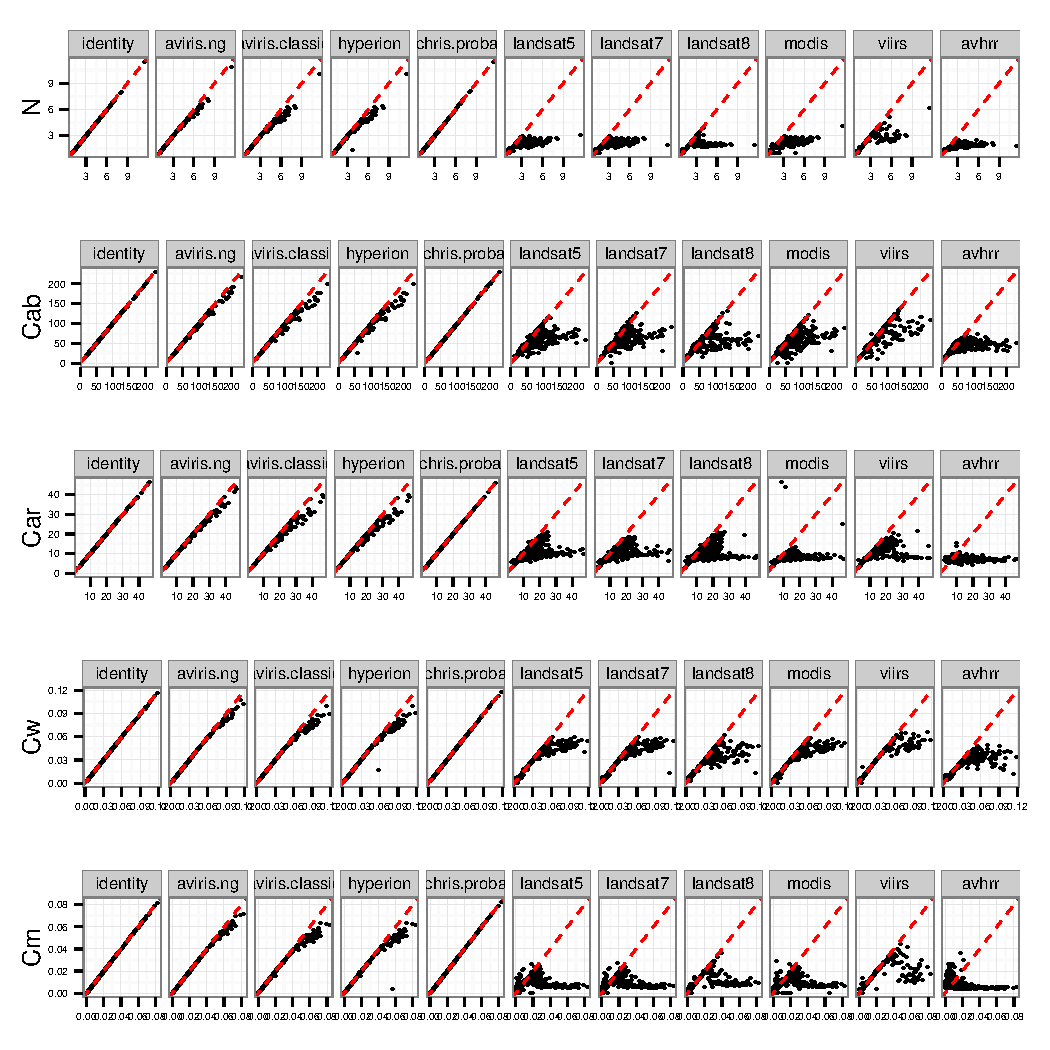
\includegraphics{figures/sensor-error}} 
  \caption{
    Parameter inversion estimates as a function of true values for the 
    spectral response functions of different sensors. The dashed red line is a 
    1:1 fit.
  }
  \label{fig:sensor-error}
\end{figure}

\subsubsection{Parameter uncertainty and covariance}

Figure \ref{fig:pairs-4} shows an example of processed output of inversions
based on full field spectra and the spectral response functions of AVIRIS NG,
Landsat 8, and MODIS. All four plots are simulated from a single set of
parameters, so differences in results are caused only by variations in the
quality of the spectra. Out of these four sensors, the smallest overall
uncertainties are in the full spectra, and the second-smallest are in the
AVIRIS NG spectra, while the uncertainties for Landsat 8 and MODIS are
comparable overall but strongly parameter dependent.  More importantly, the
shapes of parameter covariances are distinctly different between these
sensors, reflecting differences in the inversion's ability to distinguish
between parameters based on the available information.  Across all four of
these sensors, we observe negative covariance between Cw and Cm, which makes
sense given the spectral overlap between these parameter pairs in the SWIR
(Figure \ref{fig:prospectsens}). The full spectra, AVIRIS NG, and MODIS share
a strong positive covariance between N and Cm, but this covariance is largely
absent in Landsat 8, presumably because at least one Landsat band is only
affected by N and not Cm. On the other hand, Landsat has a strong negative
covariance between Cab and Car because the precise location of its visible
bands limits its ability to distinguish between these two spectrally-proximate
parameters. Similarly, MODIS has a strong negative covariance between N and
Cw, which, considered together with the strong N-Cm and Cw-Cm covariances is a
symptom of its weakness at measuring in the SWIR.

\begin{figure}[h] \centering
  \centerline{ 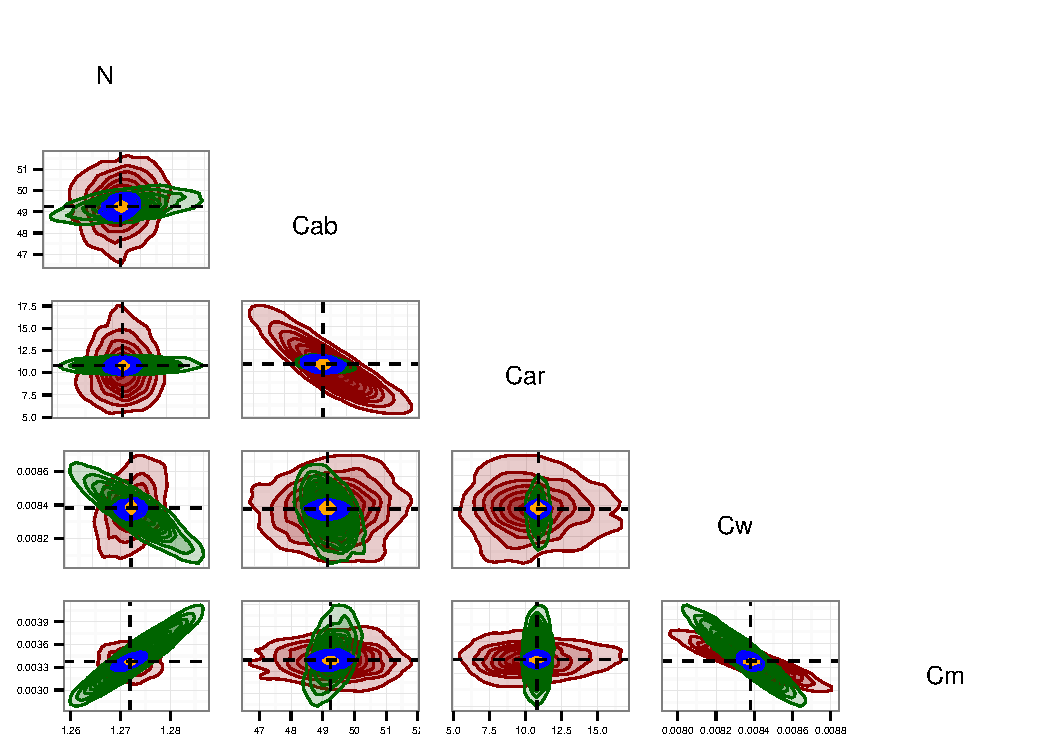
\includegraphics{figures/pairs-4}} 
  \caption{
    Joint probability distribution for parameter inversion estimates of 
    simulated spectra using the full spectra (orange) and the spectral
    response functions of AVIRIS NG (blue), MODIS (green), and Landsat 8
    (red). Dotted lines indicate true parameter values.
  }
  \label{fig:pairs-4}
\end{figure}